\let\lesson\undefined
\newcommand{\lesson}{\phantomlesson{Bài 7.}}
\setcounter{section}{2}
\section{Bài tập trắc nghiệm}
\begin{enumerate}[label=\bfseries Câu \arabic*:,leftmargin=1.5cm]
	
	
		\item \mkstar{2}
	
	{Một vật chuyển động thẳng chậm dần đều với tốc độ ban đầu $\SI{3}{\meter/\second}$ và gia tốc có độ lớn $\SI{2}{\meter/\second^2}$. Biết thời điểm ban đầu vật ở gốc tọa độ và chuyển động ngược chiều dương của trục tọa độ. Phương trình chuyển động của vật là
		\begin{mcq}(2)
			\item $x=-3t-t^2$ (m, s).
			\item $x=3t+t^2$ (m, s).
			\item $x=-3t-t^2$ (m, s).
			\item $x=-3t+t^2$ (m, s).
		\end{mcq}
	}
	\hideall
	{	\textbf{Đáp án: D.}
		
		Chọn gốc thời gian là khi vật bắt đầu chuyển động.
		
		Vì vật chuyển động chậm dần đều ngược chiều dương nên:
		\begin{equation*}
			\left\{\begin{array}{ll}{a\cdot v <0}&\\{v < 0}&\end{array}\right.\Rightarrow \left\{\begin{array}{ll}{a > 0}&\\{v < 0.}&\end{array}\right.
		\end{equation*}
		
		Kết hợp với các dữ kiện của đề bài, ta suy ra:
		\begin{equation*}
			\left\{\begin{array}{ll}{a=\SI{2}{\meter/\second^2}}&\\{v=\SI{-3}{\meter/\second} .}&\end{array}\right.
		\end{equation*}
		
		Phương trình chuyển động của vật có dạng:
		$x=-3t+t^2$ (m, s).
	}

\item \mkstar{2}\\
{Phương trình nào sau đây là phương trình tọa độ của một vật chuyển động thẳng chậm dần đều dọc theo trục $Ox$?
	\begin{mcq}(2)
		\item $s=2t-3t^2$.
		\item $x=5t^2-2t+5$.
		\item $v=4-t$.
		\item $x=2-5t-t^2$.
	\end{mcq}
	
}
\hideall{
	\textbf{Đáp án: B.}
}

	\item \mkstar{2}
	
	{ Một vật chuyển động thẳng chậm dần đều với tốc độ ban đầu $\SI{4}{\meter/\second}$ và gia tốc có độ lớn $\SI{2}{\meter/\second^2}$. Biết thời điểm ban đầu vật ở gốc tọa độ và chuyển động cùng chiều dương của trục tọa độ. Phương trình chuyển động của vật là
		\begin{mcq}(2)
			\item $x=-4t-t^2$ (m, s).
			\item $x=4t-t^2$ (m, s).
			\item $x=4t-t^2$ (m, s).
			\item $x=-4t+t^2$ (m, s).
		\end{mcq}
	}
	\hideall
	{	\textbf{Đáp án: B.}
		
		Chọn gốc thời gian là khi vật bắt đầu chuyển động.
		
		Vì vật chuyển động chậm dần đều cùng chiều dương nên:
		\begin{equation*}
			\left\{\begin{array}{ll}{a\cdot v <0}&\\{v > 0}&\end{array}\right.\Rightarrow \left\{\begin{array}{ll}{a < 0}&\\{v > 0.}&\end{array}\right.
		\end{equation*}
		
		Kết hợp với các dữ kiện của đề bài, ta suy ra:
		\begin{equation*}
			\left\{\begin{array}{ll}{a=\SI{-2}{\meter/\second^2}}&\\{v=\SI{4}{\meter/\second} .}&\end{array}\right.
		\end{equation*}
		
		Phương trình chuyển động của vật có dạng:
		$x=4t-t^2$ (m, s).
	}


\item \mkstar{3}\\
{Phương trình toạ độ của một vật chuyển động thẳng biến đổi đều là: $x = 20t^2 + 40t + 6$ (cm; s). Tính gia tốc và tính chất của chuyển động.
	\begin{mcq}(2)
		\item $\SI{40}{\centi\meter/\second^2}$; vật chuyển động nhanh dần đều.
		\item $\SI{40}{\centi\meter/\second^2}$; vật chuyển động chậm dần đều.
		\item $\SI{20}{\centi\meter/\second^2}$; vật chuyển động nhanh dần đều.
		\item $\SI{20}{\centi\meter/\second^2}$; vật chuyển động chậm dần đều.
	\end{mcq}
	
}
\hideall{
	\textbf{Đáp án: A.}\\
	$$a=\SI{40}{\centi\meter/\second^2}; v_0=\SI{40}{\meter/\second}$$
	Vì $a\cdot v_0>0$ nên vật chuyển động thẳng nhanh dần đều.
}

	\item 	\mkstar{3}\\
	{Cùng một lúc, vật thứ nhất đi từ A hướng đến B với vận tốc ban đầu $\SI{10}{\meter/\second}$, chuyển động chậm dần đều với gia tốc $\SI{0.2}{\meter/\second^2}$; vật thứ hai chuyển động nhanh dần đều, không vận tốc đầu từ B về A với gia tốc $\SI{0.4}{\meter/\second^2}$. Biết $AB = \SI{560}{\meter}$. Chọn A làm gốc tọa độ, chiều dương hướng từ A đến B, gốc thời gian là lúc hai vật bắt đầu chuyển động. Phương trình chuyển động của hai vật là
		\begin{mcq}(2)
			\item $x_1=10t-0,1t^2$ $\left(\si{\meter}\right)$; $x_2=560-0,2t^2$ $\left(\si{\meter}\right)$.
			\item $x_1=10t-0,2t^2$ $\left(\si{\meter}\right)$; $x_2=560-0,4t^2$ $\left(\si{\meter}\right)$.
			\item $x_1=10t+0,1t^2$ $\left(\si{\meter}\right)$; $x_2=560+0,2t^2$ $\left(\si{\meter}\right)$.
			\item $x_1=10t+0,2t^2$ $\left(\si{\meter}\right)$; $x_2=560+0,4t^2$ $\left(\si{\meter}\right)$.
		\end{mcq}
	
}
\hideall{
\textbf{Đáp án: A.}
}

\item \mkstar{3}\\
{Cùng một lúc ở hai điểm cách nhau $\SI{300}{\meter}$, có hai ô tô đi ngược chiều nhau. Xe thứ nhất đi từ A có tốc độ ban đầu là $\SI{10}{\meter/\second}$, xe thứ hai đi từ B với tốc độ ban đầu là $\SI{20}{\meter/\second}$. Biết xe đi từ A chuyển động nhanh dần đều, xe đi từ B chuyển động chậm dần đều và hai xe chuyển động với gia tốc có cùng độ lớn $\SI{2}{\meter/\second^2}$.
	a. Khoảng cách giữa hai xe sau $\SI{5}{\second}$ là 
	\begin{mcq}(4)
		\item $\SI{100}{\meter}$.
		\item $\SI{150}{\meter}$.
		\item $\SI{200}{\meter}$.
		\item $\SI{400}{\meter}$.
	\end{mcq}
b. Hai xe gặp nhau sau thời gian
\begin{mcq}(4)
	\item $\SI{10}{\second}$.
	\item $\SI{20}{\second}$.
	\item $\SI{30}{\second}$.
	\item $\SI{40}{\second}$.
\end{mcq}
c. Vị trí gặp nhau cách vị trí ban đầu của xe thứ nhất
\begin{mcq}(4)
	\item $\SI{100}{\meter}$.
	\item $\SI{150}{\meter}$.
	\item $\SI{200}{\meter}$.
	\item $\SI{250}{\meter}$.
\end{mcq}
}
\hideall{
\textbf{Đáp án: B-A-C.}
}



	\item \mkstar{3}
	
	{Lúc $\SI{7}{\hour}$, hai ô tô bắt đầu khởi hành từ hai điểm A, B cách nhau $\SI{2400}{\meter}$, chuyển động nhanh dần đều và ngược chiều nhau. Ô tô đi từ A có gia tốc $\SI{1}{\meter / \second \squared}$, còn ô tô đi từ B có gia tốc $\SI{2}{\meter / \second \squared}$. Chọn chiều dương hướng từ A đến B, gốc thời gian lúc $\SI{7}{\hour}$. Xác định vị trí hai xe gặp nhau.
		\begin{mcq}(4)
			\item $\SI{1600}{\meter}$.
			\item $\SI{1200}{\meter}$.
			\item $\SI{800}{\meter}$.
			\item $\SI{2400}{\meter}$.
		\end{mcq}
	}
	\hideall
	{	\textbf{Đáp án: C.}
		
		Chọn chiều dương hướng từ A đến B, gốc thời gian lúc $\SI{7}{\hour}$.
		
		Phương trình chuyển động của xe A: $x_\text A = 0,5t^2$.
		
		Phương trình chuyển động của xe B: $x_\text B=-t^2 + 2400$.
		
		Hai xe gặp nhau: $x_\text A = x_\text B \Rightarrow t = \SI{40}{\second} \Rightarrow x=\SI{800}{\meter}$.
	}

\item \mkstar{3}\\
{Lúc $\SI{1}{\hour}$, một xe qua A với tốc độ $\SI{10}{\meter/\second}$, chuyển động nhanh dần đều với gia tốc $\SI{1}{\meter/\second^2}$ đuổi theo một xe đạp đang chuyển động nhanh dần đều qua B với tốc độ đầu là $\SI{2}{\meter/\second}$ và với gia tốc là $\SI{0.5}{\meter/\second^2}$. Sau $\SI{20}{\second}$ thì xe đuổi kịp xe đạp. Tính khoảng cách AB.
\begin{mcq}(4)
	\item $\SI{300}{\meter}$.
	\item $\SI{250}{\meter}$.
	\item $\SI{200}{\meter}$.
	\item $\SI{260}{\meter}$.
\end{mcq}
}
\hideall{
\textbf{Đáp án: D.}
}

\item \mkstar{3}\\
{Vật (1) xuất phát lúc 7h30 từ A chuyển động thẳng nhanh dần đều với tốc độ ban đầu $\SI{2}{\meter/\second}$, gia tốc $\SI{1}{\meter/\second^2}$ hướng về B. Sau 2 giây, vật (2) xuất phát từ B chuyển động thẳng nhanh dần đều không vận tốc đầu về A với gia tốc $\SI{2}{\meter/\second^2}$. Khoảng cách $AB = \SI{134}{\meter}$.\\
	a. Tìm thời gian và vị trí hai vật gặp nhau.
	\begin{mcq}(4)
		\item $t=\SI{5}{\second}$, $x_1=\SI{70}{\meter}$.
		\item $t=\SI{10}{\second}$, $x_1=\SI{50}{\meter}$.
		\item $t=\SI{10}{\second}$, $x_1=\SI{70}{\meter}$.
		\item$t=\SI{5}{\second}$, $x_1=\SI{50}{\meter}$.
	\end{mcq}
b. Sau bao lâu kể từ lúc bắt đầu chuyển động 2 vật cách nhau $\SI{50}{\meter}$?
\begin{mcq}(4)
	\item $\SI{15}{\second}$ và $\SI{11.6}{\second}$.
	\item $\SI{8}{\second}$ và $\SI{16}{\second}$.
	\item $\SI{15}{\second}$ và $\SI{16}{\second}$.
	\item $\SI{8}{\second}$ và $\SI{11.6}{\second}$.
\end{mcq}
}
\hideall{
\textbf{Đáp án: C-D.}
}

\end{enumerate}

\section{Bài tập tự luận}
\begin{enumerate}[label=\bfseries Bài \arabic*:,leftmargin=1.5cm]
\item \mkstar{2}\\
Một chất điểm chuyển động dọc theo trục $Ox$ với phương trình $x=5+10t-0,25t^2$; trong đó $x$ tính bằng mét, $t$ tính bằng giây.
\begin{enumerate}
	\item Xác định gia tốc và vận tốc của chất điểm. Chuyển động của chất điểm là loại chuyển động nào?
	\item Tìm vận tốc tức thời của chất điểm lúc $t=\SI{4}{\second}$.
\end{enumerate}
\hideall{
\begin{enumerate}[label=\alph*)]
	\item Gia tốc của chất điểm $a=\SI{-0.5}{\meter/\second^2}$.\\
	Vận tốc đầu của chất điểm $v_0=\SI{10}{\meter/\second}$.\\
	Do $av_0<0$ nên chất điểm chuyển động thẳng chậm dần đều.
	\item Vận tốc tức thời của chất điểm lúc $t=\SI{4}{\second}$:
	$$v=v_0+at=\SI{10}{\meter/\second}+\left(\SI{-0.5}{\meter/\second^2}\right)\cdot\left(\SI{4}{\second}\right)=\SI{8}{\meter/\second}.$$
\end{enumerate}
}

\item \mkstar{3}\\
Đồ thị chuyển động của hai xe được biểu diễn như hình \ref{fig:TP010-P-1}.
\begin{center}
	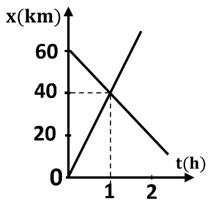
\includegraphics[width=0.25\linewidth]{../figs/VN10-2023-PH-TP010-P-1}
	\captionof{figure}{}
	\label{fig:TP010-P-1}
\end{center}
\begin{enumerate}[label=\alph*)]
	\item Nêu tính chất chuyển động của hai xe.
	\item Dựa vào đồ thị, xác định vị trí của hai xe tại thời điểm $\SI{1.5}{\hour}$.
\end{enumerate}
\hideall{
	\begin{enumerate}[label=\alph*)]
		\item Xe 1 chuyển động từ gốc toạ độ, chuyển động thẳng đều theo chiều dương với tốc độ $v_1=\SI{40}{\kilo\meter/\hour}$.\\
		Xe 2 chuyển động từ vị trí cách gốc toạ độ $\SI{60}{\kilo\meter}$, chuyển động thẳng đều theo chiều âm với tốc độ $v_2=\SI{20}{\kilo\meter/\hour}$.
		\item Sau thời gian $\SI{1.5}{\hour}$ xe 1 ở vị trí cách gốc toạ độ $\SI{60}{\kilo\meter}$, xe 2 ở vị trí cách gốc toạ độ $\SI{30}{\kilo\meter}$.
	\end{enumerate}
}	
	


\item \mkstar{3}\\
Một ô tô khởi hành từ A chuyển động thẳng nhanh dần đều đến B cách A $\SI{3}{\kilo\meter}$. Trong giây thứ 6 xe chạy được quãng đường $\SI{11}{\meter}$.
\begin{enumerate}[label=\alph*)]
	\item Tính gia tốc của ô tô và thời gian chay $\SI{1}{\kilo\meter}$ cuối cùng.
	\item Viết phương trình chuyển động của ô tô. Chọn gốc toạ độ tại A, gốc thời gian lúc khởi hành, chiều dương ngược chiều chuyển động của xe.
\end{enumerate}
\hideall{
\begin{enumerate}[label=\alph*)]
	\item Trong giây thứ 6 ô tô chạy được quãng đường $\SI{11}{\meter}$:
	$$\dfrac{1}{2}a\cdot6^2-\dfrac{1}{2}a\cdot5^2=\SI{11}{\meter}\Rightarrow a=\SI{2}{\meter/\second^2}.$$
	Thời gian ô tô chạy từ A đến B:
	$$t_\text{AB}=\sqrt{\dfrac{2\text{AB}}{a}}=\xsi{10\sqrt{30}}{\second}.$$
	Thời gian ô tô chạy $\SI{2}{\kilo\meter}$ đầu tiên:
	$$t=\sqrt{\dfrac{2s}{a}}=\xsi{20\sqrt{5}}{\second}.$$
	Thời gian ô tô chạy $\SI{1}{\kilo\meter}$ cuối cùng:
	$$\Delta t=t_\text{AB}-t\approx\SI{10.05}{\second}.$$
	\item Chọn gốc toạ độ tại A, gốc thời gian lúc khởi hành, chiều dương là ngược chiều chuyển động của ô tô.\\
	Phương trình chuyển động của ô tô:
	$$x=x_0+v_0t+\dfrac{1}{2}at^2=\dfrac{1}{2}\cdot\left(-2\right)t^2=-t^2\quad \left(\si{\meter}, \si{\second}\right).$$
\end{enumerate}
}

\item \mkstar{3}\\
{Cùng một lúc, từ hai địa điểm A và B cách nhau $\SI{50}{m}$ có hai vật chuyển động ngược chiều để gặp nhau. Vật thứ nhất xuất phát từ A chuyển động đều với vận tốc $\SI{5}{m/s}$, vật thứ hai xuất phát từ B chuyển động nhanh dần đều không vận tốc đầu với gia tốc $\SI{2}{m/s}^2$. Chọn trục $Ox$ trùng đường thẳng AB, gốc tọa độ tại A, chiều dương từ A đến B, gốc thời gian là lúc xuất phát
	\begin{enumerate}[label=\alph*.]
		\item Viết phương trình chuyển động của mỗi vật.
		\item Xác định thời điểm và vị trí hai gặp nhau.
		\item Xác định thời điểm mà tại đó hai vật có độ lớn vận tốc bằng nhau.
	\end{enumerate}
}
\hideall{
	Chọn chiều dương là chiều chuyển động của xe A, gốc tọa độ ở A, gốc thời gian từ lúc xe hai xe bắt đầu chuyển động. 
	\begin{enumerate}[label=\alph*.]
		\item Phương trình chuyển động của 2 xe lần lượt là:
		
		$$x_\text{1} = x_{10}+v_{1}t = v_{1}t.$$
		
		$$x_\text{2} = x_{20} + v_{20}t +\dfrac{1}{2}a_2t^2 = x_{20} +\dfrac{1}{2}a_2 t^2.$$
		\item Hai xe gặp nhau thì:
		
		$$x_{1} = x_{2}.$$
		$$\Leftrightarrow  v_{10}t= x_{20} +\dfrac{1}{2}a_2 t^2.$$
		Thay các giá trị số 
		$$v_{1}=\SI{5}{\meter/\second},\quad x_{20}=\SI{50}{\meter},\quad a_2=\SI{-2}{\meter/\second^{2}},$$
		và giải phương trình trên, ta thu được hai nghiệm $t=\SI{0}{\second}$ và $t =\SI{5}{s}.$ Ta chọn nghiệm $t =\SI{5}{s}$ do ta chỉ xét thời gian sau khi hai xe đã chuyển động. 
		
		Vị trí gặp nhau của hai xe
		$$x_1\simeq x_2=v_{1}t=\SI{5}{\meter/\second}\cdot\SI{5}{\second}=\SI{25}{\meter}.$$
		Vậy hai xe gặp nhau sau $\SI{5}{s}$ và cách A $\SI{25}{m}.$
		\item Phương trình vận tốc của xe thứ hai  là
		
		$$v_{2} = v_{20} +a_2t=a_2t$$
		
		Hai xe có cùng độ lớn vận tốc
		$$\left|v_1\right|=\left|v_2\right|\quad\Rightarrow\quad v_1=a_2t\quad\Rightarrow\quad t=\left|\dfrac{v_1}{a_2}\right|=\left|\dfrac{\SI{5}{\meter/\second}}{\SI{-2}{\meter/\second^{2}}}\right|=\SI{2.5}{\second}.$$
	\end{enumerate}
}

\item \mkstar{3}\\
{Hai vật cùng xuất phát một lúc tại A, chuyển động cùng chiều. Vật thứ nhất chuyển động đều với vận tốc $v_1 = \SI{20}{m/s}$, vật thứ hai chuyển động thẳng nhanh dần đều với vận tốc ban đầu bằng không và gia tốc $\SI{0,4}{m/s}^2$. Chọn chiều dương là chiều chuyển động, gốc tọa độ O tại A, gốc thời gian là lúc xuất phát.
	\begin{enumerate}[label=\alph*)]
		\item Xác định thời điểm và vị trí hai xe gặp nhau.
		\item Viết phương trình vận tốc của vật thứ hai. Xác định khoảng cách giữa hai vật tại thời điểm chúng có vận tốc bằng nhau.
	\end{enumerate}
}
\hideall{
	\begin{enumerate}[label=\alph*)]
		\item Phương trình chuyển động:
		$$x_1 = 20t.$$
		$$x_2 = \text{0,2}t^2.$$
		
		Khi hai vật gặp nhau thì:
		
		$$x_1 =x_2 \quad\Rightarrow\quad 20\;t = \text{0,2}\;t^2\quad\Rightarrow\quad t =\SI{0}{\second}\quad\vee\quad t =\SI{100}{s}.$$
		Ta chọn nghiệm $t =\SI{100}{s}$ ứng với thời điểm hai xe gặp lại nhau. 
		
		Vị trí hai xe gặp lại nhau 
		$$x_1 =x_2 =20t=\SI{2000}{m}.$$
		\item Phương trình vận tốc của vật thứ hai
		$$v_2 =v_{20}+a_2t=\text{0,4}\;t\ \text{m/s}.$$
		
		Thời điểm lúc hai vật có vận tốc bằng nhau: 
		$$v_2 =\text{0,4}\;t = 20 \quad\Rightarrow\quad t = \SI{50}{s}.$$
		
		Tọa độ các vật lúc đó: 
		
		$$x_1 = 20\;t = \SI{1000}{m};\quad x_2 = \text{0,2}\;t^2 = \SI{500}{m}.$$
		
		Khoảng cách giữa hai vật: 
		
		$$d= \left|x_1 - x_2\right| =\SI{500}{m}.$$
	\end{enumerate}
}


\item \mkstar{4}


{
	Một ôtô chạy đều trên một con đường thẳng với tốc độ $\SI{25}{\meter/\second}$ (vượt quá tốc độ) thì bị cảnh sát giao thông phát hiện. Chỉ sau $\SI{2}{\second}$ khi ôtô đi qua một cảnh sát, anh cảnh sát này bắt đầu đuổi theo với gia tốc không đổi và bằng $\SI{6}{\meter/\second^2}$. Tìm thời điểm và vị trí anh cảnh sát đuổi kịp ô tô.
}

\hideall
{	
	Chọn chiều dương là chiều chuyển động của xe ô tô và anh cảnh sát, gốc tọa tọa là vị trí của anh cảnh sát đang đứng, gốc thời gian là thời điểm cảnh sát bắt đầu đuổi theo xe.
	
	Phương trình chuyển động của xe ôtô là:
	
	$$x=x_0+v_0(t+2)=25(t+2)\ \text{(m; s)}.$$
	
	Phương trình chuyển động của anh cảnh sát là:
	
	$$x'=x_0'+v_0't+\dfrac{1}{2}at^2=3t^2\ \text{(m; s)}.$$
	
	Thời điểm anh cảnh sát đuổi kịp xe ôtô là:
	
	$$x=x'\Rightarrow 25(t+2)=3t^2\Rightarrow t=\SI{10}{\second}.$$
	
	Vị trí anh cảnh sát đuổi kịp xe ôtô là:
	
	$$x'=3t^2=\SI{300}{\meter}.$$
}
\item \mkstar{4}


{
	Hai chất điểm A và B cách nhau $\SI{60}{\meter}$. Tại thời điểm $t=0$ chất điểm A chuyển động về phía B với vận tốc không đổi $\SI{12}{\meter / \second}$. Cùng thời điểm đó chất điểm B cũng chuyển động với gia tốc $\SI{2}{\meter / \second \squared}$ theo hướng ra xa A. Tìm thời điểm mà khoảng cách giữa A và B là ngắn nhất.
}

\hideall
{Chọn chiều dương của trục $\text O x$ cùng hướng chuyển động của A và B, gốc O tại vị trí ban đầu của A. Gốc thời gian là lúc vật A và B bắt đầu chuyển động.
	
	Phương trình chuyển động của A: $x_\text A = 12t$.
	
	Phương trình chuyển động của B: $x_\text B = t^2 + 60$.
	
	Khoảng cách giữa A và B: $|x_\text B - x_\text A |=|t^2+60-12t|=|(t-6)^2+24|$.
	
	Khoảng cách này nhỏ nhất khi $(t-6)^2 = 0 \Rightarrow t=\SI{6}{\second}$.
}
\end{enumerate}
